As with the original Prophet 600 firmware, there are two modes of operation, a \textbf{Preset} mode and a \textbf{Live} mode. The user can change between the two by pressing the \textbf{Preset} button, see section \ref{datapad}. 

The idea of the live mode (LED of preset button is off) is that the patch that is playing corresponds to exactly the parameters as currently set by all dials, switches and additional patch parameters. The synth produces the sound as set and seen. In the preset mode (LED of preset button is on), in contrast, the patch parameter as stored in the patch memory are applied. The synth produces the the sound of the preset. Still, once a dial or a switch on the panel or an additional parameter is changed, this change will take effect. In this case a "mixed state" applies, partly patch (untouched controls) and partly panel controls (touched controls). The user can then store the current sound in the same patch or a different patch (See section \ref{loadstorepatches}). The patch will be stored as heard. 

\textbf{Preset patch vs. preset panel mode}

In preset mode the default setup is preset patch mode in which the number pad is used to select and load presets. However, in preset mode the user can also decide to switch to preset panel mode in which the number pad selects additional patch parameters similar to live mode. To do so, press \textbf{To Tape}. The LED is active. To leave the preset panel mode, press To Tape again. 

\textbf{Pick-me-up mode in preset panel mode}

The fact that the controls in preset modes may not correspond to the current active parameter values has two disadvantages. Firstly, once a control is touched it is immediately applied, irrespectively of where it is currently pointing to and how far away that value is from the one used in the patch you are hearing. This may lead to unwanted, disruptive sound changes. Secondly, it may be difficult or cumbersome to retrieve an original patch value once it is changed using a control. Therefore the upgraded Prophet 600 supports a \textit{pick-me-up} control logic for dials in preset panel mode. It works as follows:

If you touch and change a dial the display indicates if the current active value is below the current dial position (arrow on the left) or above it (arrows on the right). As long a these arrows are shown the value of the dial will not be applied, it is not "picked up". Once you touch the current active value closely enough the display switches to showing the numerical value instead, indicating that the dial is "picked up". From that moment on all movements of the dial are always applied. The logic is shown shcematically below.

\scalebox{0.4}{
  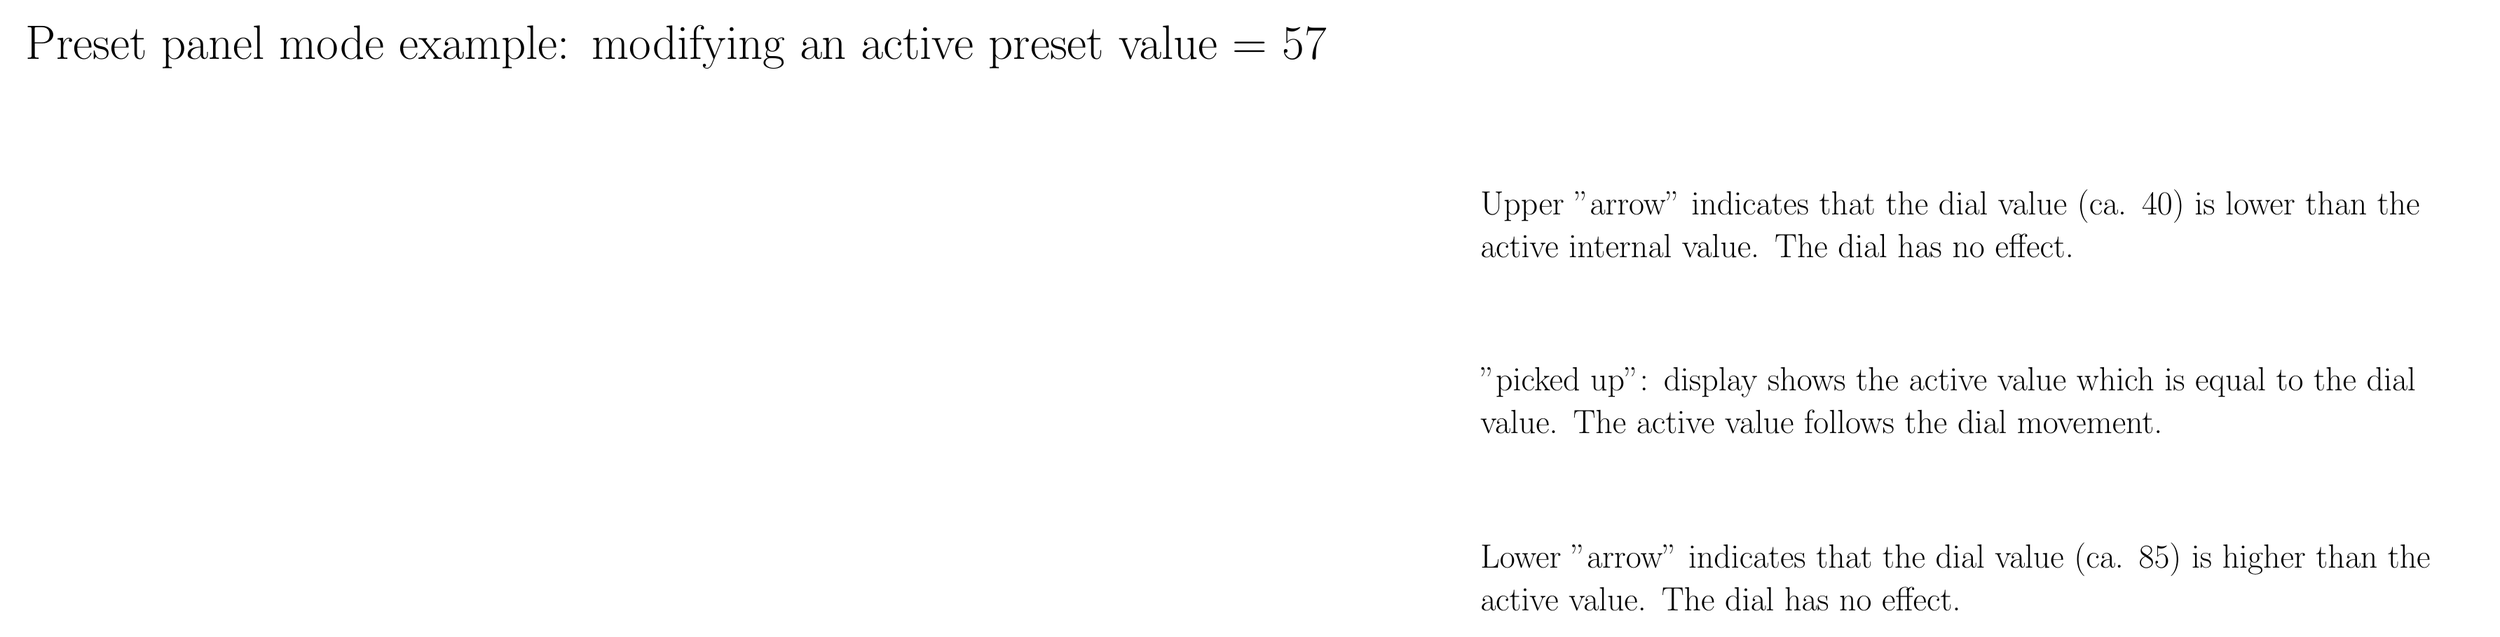
\begin{tikzpicture}[scale=0.8]
  \node[font=\fontsize{24}{22}\selectfont, align=left, outer sep=0.5mm, anchor = west, text width=40cm] at (3cm,20cm) {Preset panel mode example: modifying an active preset value = 57};
    \upperbuttons{6.5cm,7.5cm}{PT}{}

    \prophetpot{26cm,8cm}{}{345}
    \prophetdisplay{32cm,8cm}{567}{}{}
    \node[font=\fontsize{18}{22}\selectfont, align=left, anchor = west, text width=18cm] at (36cm,8cm) {Lower "arrow" indicates that the dial value (ca. 85) is higher than the active value. The dial has no effect.};

    \prophetpot{26cm,12cm}{}{65}
    \prophetdisplay{32cm,12cm}{13467}{123}{}
    \node[font=\fontsize{18}{22}\selectfont, align=left, anchor = west, text width=18cm] at (36cm,12cm) {"picked up": display shows the active value which is equal to the dial value. The active value follows the dial movement.};

    \prophetpot{26cm,16cm}{}{125}
    \prophetdisplay{32cm,16cm}{}{237}{}
    \node[font=\fontsize{18}{22}\selectfont, align=left, anchor = west, text width=18cm] at (36cm,16cm) {Upper "arrow" indicates that the dial value (ca. 40) is lower than the active internal value. The dial has no effect.};
    
  \end{tikzpicture}
}

The pick-me-up mechanism avoids disruptive value changes and provides a means to dial the current panel into the patch you're hearing. Note, however, that is important to observe the display and current pick-up status od dials to avoid confusion. If a direct application of dials is needed then press To Tape to switch back to standard preset mode.

There is no pick-up mechanism for switches on the panel and the mechanim is also irrelevant for additional patch parameters as there is no conflict between physical controls and interally applied values. Furthermore, the logic on applies only to patch parameters. It is therefore not applied to master tune, (master) volume, pitch bend and modulation wheel.
